\chapter{Contextualização}

A digitalização do setor financeiro ampliou o acesso dos usuários a contas bancárias, cartões e outros serviços oferecidos por diferentes instituições. Embora esse cenário proporcione maior conveniência, também contribui para a fragmentação da vida financeira, fazendo com que o acompanhamento de saldos, despesas e compromissos frequentemente dependa da consulta a diferentes aplicativos e da interpretação de informações provenientes de múltiplas fontes.

Apesar da disponibilidade desses dados, seu acompanhamento ainda depende, em grande parte, da iniciativa do próprio usuário, uma vez que muitas soluções permanecem centradas em \textit{dashboards}, extratos e gráficos que exigem consultas ativas. Além disso, a existência das informações não garante que elas sejam facilmente compreendidas ou utilizadas na tomada de decisões. O baixo nível de letramento financeiro digital observado em estudos internacionais realizados pela \textit{Organisation for Economic Co-operation and Development} reforça a necessidade de soluções que simplifiquem a interpretação das informações financeiras (OECD, 2023).

Nesse contexto, o \textit{Open Finance} possibilita o compartilhamento padronizado de dados financeiros entre instituições autorizadas, mediante consentimento do titular, criando condições para que informações anteriormente dispersas possam ser utilizadas de forma integrada (Banco Central do Brasil; Conselho Monetário Nacional, 2020). Entretanto, essa infraestrutura, isoladamente, não garante que os dados sejam transformados em informações compreensíveis, contextualizadas e úteis para a tomada de decisões pelo usuário.

Paralelamente, a ampla utilização de plataformas de mensageria cria oportunidades para aproximar os serviços financeiros da rotina dos usuários. Nesse sentido, o \textit{WhatsApp} apresenta-se como um canal inicial adequado para a solução, por permitir que a interação ocorra em um ambiente já familiar ao público (Meta Platforms, Inc., [s. d.]). Contudo, vincular toda a operação do sistema a uma única plataforma representaria uma dependência tecnológica e comercial em relação ao provedor responsável pelo canal de comunicação, podendo limitar sua capacidade de expansão e adaptação.

Diante desse cenário, este trabalho apresenta o desenvolvimento do EIGAM, uma solução de assistência financeira inteligente, preditiva e conversacional que interage com os usuários por meio de plataformas de mensageria. O \textit{WhatsApp} foi adotado como principal canal de interação, e a arquitetura foi estruturada de forma desacoplada da plataforma de comunicação, o que permitiu integrar também o \textit{Telegram} e uma conversa no painel \textit{web} do titular sem alterações no núcleo funcional.

A solução integra dados obtidos via \textit{Open Finance} a técnicas de análise preditiva e a um assistente conversacional baseado em modelos de linguagem e em recuperação de contexto, transformando dados financeiros dispersos em informações contextualizadas e úteis. Além de responder a consultas em linguagem natural, a solução atua de forma proativa por meio de avisos sobre limites de gasto, cobranças duplicadas e transações atípicas, de metas financeiras e de resumos periódicos, apoiando a tomada de decisões financeiras e observando os requisitos de privacidade e proteção de dados previstos na Lei Geral de Proteção de Dados Pessoais (LGPD) (Brasil, 2018).

\section{Objetivo}

Desenvolver uma solução de assistência financeira inteligente, preditiva e conversacional, capaz de integrar dados provenientes do \textit{Open Finance} e fornecer ao usuário consultas, análises, previsões, alertas e orientações personalizadas por meio de plataformas de mensageria, utilizando o \textit{WhatsApp} como principal canal de interação e mantendo a arquitetura desacoplada da plataforma de comunicação, de modo a permitir a integração com outros serviços de mensageria e reduzir a dependência de um único provedor.

Para atingir esse objetivo geral, foram definidos os seguintes objetivos específicos:

\begin{alineas}
    \item integrar as contas bancárias do usuário por meio do \textit{Open Finance}, mediante consentimento;
    \item responder a consultas financeiras em linguagem natural, com valores obtidos de dados estruturados e não gerados pelo modelo de linguagem;
    \item emitir avisos, projeções e resumos de forma proativa;
    \item garantir a proteção dos dados e o exercício dos direitos do titular previstos na LGPD por meio da própria conversa;
    \item medir a qualidade da solução por testes automatizados, conjuntos de referência, teste de carga e teste retrospectivo.
\end{alineas}

\section{Público-alvo}

O público-alvo do negócio é formado, principalmente, por adultos economicamente ativos que já utilizam serviços bancários digitais e buscam maior controle sobre sua vida financeira de forma simples, prática e acessível. Enquadram-se nesse perfil estudantes, trabalhadores assalariados, autônomos, microempreendedores e demais usuários que desejam acompanhar gastos, organizar o orçamento, prever compromissos financeiros e transformar dados bancários em informações úteis para decisões do dia a dia.

As estratégias do negócio devem ser direcionadas especialmente a pessoas que já utilizam plataformas de mensageria como canais recorrentes de comunicação, aproveitando a familiaridade e a presença desses serviços na rotina cotidiana para reduzir barreiras de adoção tecnológica. O \textit{WhatsApp} é o principal meio de acesso ao EIGAM, aproveitando os recursos disponibilizados pela \textit{WhatsApp Business Platform}. Entretanto, a experiência não ficou restrita a esse serviço: a arquitetura permitiu incorporar o \textit{Telegram} como segundo canal e um painel \textit{web} que estende a conversa.

Além disso, como a proposta depende da integração com dados financeiros compartilhados mediante consentimento no ecossistema de \textit{Open Finance}, o serviço tende a ser especialmente relevante para usuários que desejam centralizar informações bancárias e receber análises e orientações personalizadas em linguagem natural, sem depender do acesso recorrente a uma plataforma \textit{web} específica.

\subsection{Personas}

As personas consistem em perfis fictícios elaborados com base nas características, comportamentos, necessidades e dificuldades do público que se pretende atender. Sua utilização no projeto permite compreender com maior profundidade os diferentes tipos de usuários, suas expectativas em relação à solução proposta e a forma como interagem com tecnologias voltadas à organização financeira. A partir dessa construção, torna-se possível orientar decisões de desenvolvimento com maior foco na experiência do usuário, na usabilidade e na adequação das funcionalidades ao contexto real de uso. Neste trabalho, foram definidas três personas que representam perfis contrastantes, mas compatíveis com o público-alvo da solução, conforme apresentado nas Figuras \ref{fig:persona1}, \ref{fig:persona2} e \ref{fig:persona3}.

\begin{figure}[htbp]
    \centering
    \caption{Persona 1 - Mathias Lima}
    \label{fig:persona1}
    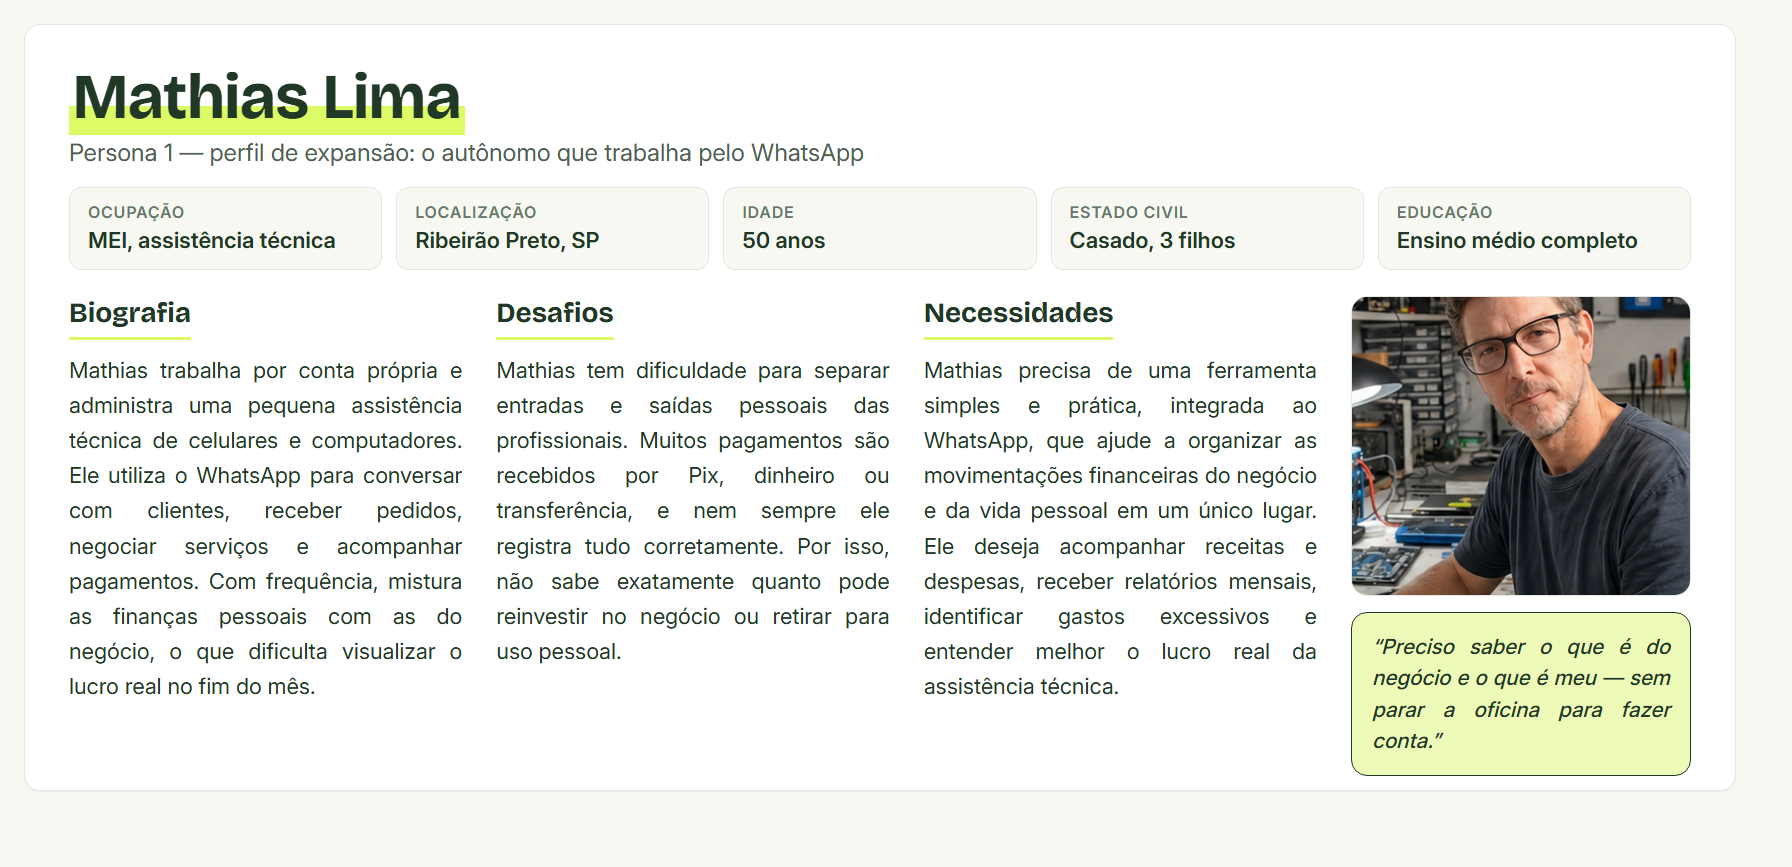
\includegraphics[width=0.9\textwidth]{images/persona_1.png}
    \authorssource
\end{figure}

\begin{figure}[htbp]
    \centering
    \caption{Persona 2 - Márcio Júnior}
    \label{fig:persona2}
    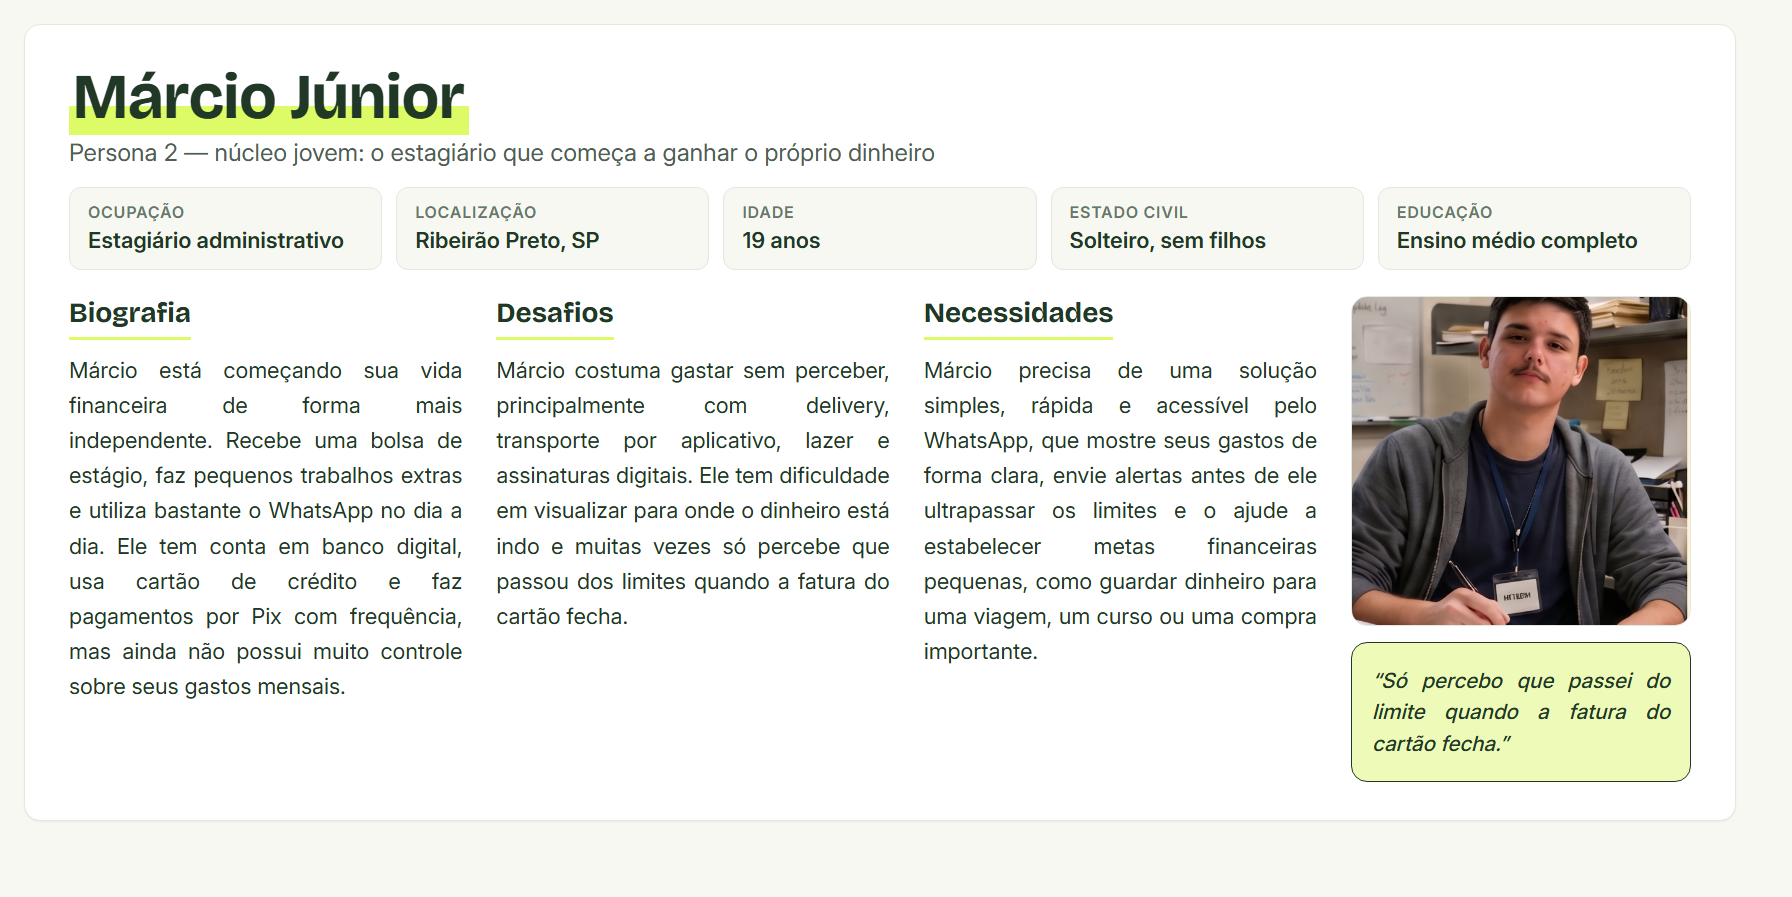
\includegraphics[width=0.9\textwidth]{images/persona_2.png}
    \authorssource
\end{figure}

\begin{figure}[htbp]
    \centering
    \caption{Persona 3 - Vitoria Moreira}
    \label{fig:persona3}
    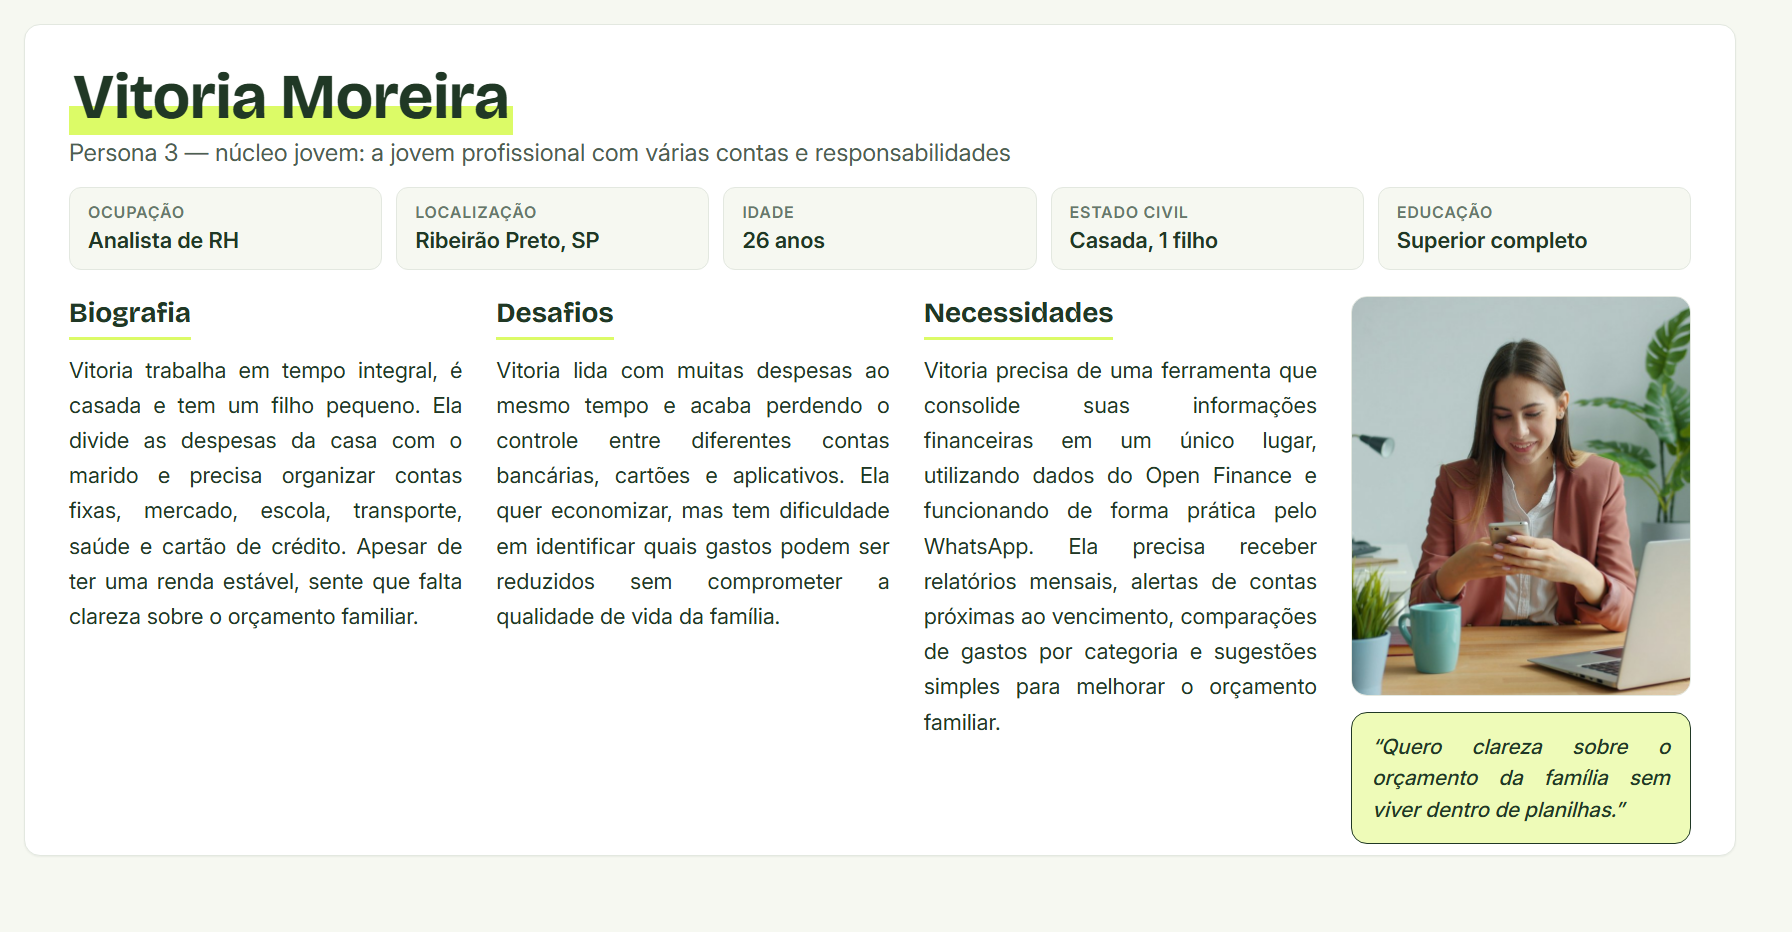
\includegraphics[width=0.9\textwidth]{images/persona_3.png}
    \authorssource
\end{figure}

\section{Conceito do produto}

O produto desenvolvido consiste em uma solução de assistência financeira inteligente, preditiva e conversacional denominada EIGAM, desenvolvida para auxiliar os usuários no acompanhamento e na compreensão de sua vida financeira por meio de plataformas de mensageria. Sua principal finalidade é atender necessidades relacionadas à organização do orçamento, compreensão dos hábitos de consumo, acompanhamento do histórico bancário, identificação de padrões de gastos, antecipação de possíveis cenários financeiros e apoio à tomada de decisões no cotidiano.

Para isso, a solução utiliza dados financeiros compartilhados pelo usuário por meio do ecossistema de \textit{Open Finance}, que possibilita o compartilhamento padronizado de informações entre instituições autorizadas mediante consentimento do titular. A integração desses dados permite consolidar informações provenientes de diferentes instituições financeiras e utilizá-las como base para os mecanismos de análise e inteligência da plataforma, reduzindo a necessidade de inserção manual de movimentações pelo usuário.

Como diferencial, o produto combina três elementos centrais em uma única experiência: a centralização de dados financeiros, a análise preditiva personalizada e a interação conversacional em linguagem natural. Em vez de exigir acesso recorrente a \textit{dashboards}, extratos e telas específicas, a solução disponibiliza consultas, análises, avisos e orientações diretamente nos canais de comunicação utilizados pelo usuário, aproximando o acompanhamento financeiro de sua rotina.

O \textit{WhatsApp} foi adotado como principal canal de comunicação com o EIGAM, aproveitando sua ampla utilização e os recursos oferecidos pela \textit{WhatsApp Business Platform}. Entretanto, o produto não foi concebido como uma solução de vínculo exclusivo a esse mensageiro. A arquitetura separa as regras de negócio, os mecanismos de análise financeira e os recursos de inteligência artificial da camada responsável pela comunicação com cada plataforma de mensageria.

Para isso, foi construída uma camada de abstração responsável por padronizar a comunicação entre os diferentes canais e o núcleo da aplicação. As mensagens recebidas pelas plataformas integradas são convertidas para uma representação interna comum antes de serem processadas pelas funcionalidades do EIGAM. De maneira semelhante, as respostas produzidas pelo sistema são encaminhadas ao adaptador do canal utilizado, responsável por adaptá-las às características e aos recursos oferecidos por cada plataforma.

Essa estratégia permitiu incorporar o \textit{Telegram} e a conversa no painel \textit{web} por meio de novos adaptadores, sem modificar os serviços responsáveis pelo processamento de dados financeiros, análise preditiva, inteligência artificial e demais regras de negócio. Dessa forma, o \textit{WhatsApp} funciona como o principal canal de acesso à solução, e não como uma dependência estrutural de seu funcionamento.

A adoção dessa arquitetura também busca reduzir riscos associados à dependência de um único fornecedor externo. Alterações em políticas de utilização, modelos de cobrança, disponibilidade de APIs ou restrições técnicas impostas por uma determinada plataforma de mensageria podem afetar soluções fortemente acopladas a ela. Ao possibilitar a integração com diferentes canais, o EIGAM aumenta sua flexibilidade tecnológica e sua capacidade de adaptação diante de mudanças externas. Durante o desenvolvimento, esse risco se materializou: a Meta passou a cobrar mensagens de serviço que antes eram gratuitas, e a arquitetura permitiu responder à mudança sem alterar o núcleo do produto.

A partir dos dados financeiros integrados, a solução oferece não apenas consultas realizadas pelo usuário, mas também uma atuação proativa. O sistema analisa o histórico financeiro para identificar padrões, recorrências e comportamentos relevantes, e envia avisos relacionados, por exemplo, a limites de gasto, cobranças duplicadas, transações atípicas, aumento de gasto em uma categoria e acompanhamento de metas. Dessa forma, o acompanhamento financeiro deixa de depender exclusivamente da iniciativa do usuário.

A camada conversacional, por sua vez, permite que essas informações sejam acessadas por meio de linguagem natural. Em vez de depender da interpretação direta de gráficos, extratos ou indicadores, o usuário realiza consultas relacionadas ao seu contexto financeiro e recebe informações apresentadas de maneira acessível e contextualizada, acompanhadas de imagens quando a resposta pede uma visão de conjunto. A combinação entre integração de dados, análise preditiva e interação conversacional transforma informações financeiras previamente dispersas em conhecimento aplicável às decisões cotidianas.

Entre os principais riscos do produto identificados na concepção, destacam-se a dependência do consentimento do usuário e da disponibilidade das integrações com instituições participantes do \textit{Open Finance}, os desafios relacionados à privacidade e à proteção de dados financeiros e a necessidade de garantir interpretações confiáveis por parte dos mecanismos de inteligência artificial, reduzindo respostas imprecisas ou excessivamente genéricas.

Também devem ser considerados os riscos relacionados à utilização de serviços externos de mensageria, cujas políticas, custos, interfaces de programação e condições de utilização podem sofrer alterações ao longo do tempo. Entretanto, diferentemente de uma solução exclusivamente vinculada a uma única plataforma, a arquitetura multicanal adotada mitiga esse risco por meio do desacoplamento entre a camada de comunicação e o núcleo funcional do EIGAM. Dessa forma, o sucesso do produto depende não apenas da qualidade técnica da solução, mas também de sua interoperabilidade, capacidade de evolução, conformidade regulatória, segurança da informação e construção de confiança na interação com o usuário.

